\section{Ergebnisse} % (fold)
\label{sec:ergebnisse}

  \subsection{Stabilitätsanalyse} % (fold)
  \label{sub:stabilitätsanalyse}

    Um die verschiedenen Integratoren auf ihre Genauigkeit und Stabilität hin zu untersuchen wurde ein bekanntes, analytisch lösbares Standardszenario simuliert, in diesem Fall das der Erde, die im Schwerefeld der Sonne kreist.
    Die Anfangswerte wurden dabei so gewählt, dass sie dem wirklichen Verlauf möglichst nahe kommen, so dass die Punktmasse Kreisbahnen um die Sonne beschreibt.
    Ein Integrator wird hier als stabil bezeichnet, wenn seine Lösungen beschränkt bleiben.
    Die Gesamtenergie des Systems erweist sich gutes Maß um die Stabilität einzuschätzen, da sie in gravitativ wechselwirkenden Systemen eine Erhaltungsgröße darstellt.
    Ist ein Integrator instabil, so wird sich die Gesamtenergie $E$ mit der Zeit verändern.
    Abbildung \ref{fig:sun_earth2} zeigt den Verlauf der Erdbahnkurve über mehrere Jahre für verschieden Integrationsmethoden.
    Wie man sieht, wächst die Lösung des expliziten Euler-Algorithmus mit jedem Integrationsschritt weiter an, der Planet entfernt sich immer weiter von der Sonne.
    Dieses Verhalten deckt sich gut mit der bekannten Charakteristik des Vorwärts-Euler-Integrators.
    Das Anwachsen der großen Halbachse ist mit einer Zunahme der Gesamtenergie verbunden, deren zeitliche Entwicklung in Diagramm \ref{fig:e2} dargestellt ist.
    Während die anderen Integratortypen vergleichsweise konstante Energiewerte über einen Zeitraum von $200\,\m{a}$ ausfweisen, steigt die des Euler-Integrators bereits in den ersten Jahren sehr stark an.
    Am Ende des betrachteten Bereichs geht $E$ langsam gegen Null, was einer ungebundenen Bewegung, beziehungsweise einer sehr großen Entfernung zum Stern entspricht.
    Ähnliches Verhalten ist auch beispielsweise bei der Berechnung des Federschwingers zu beobachten.

    Der symplektische Euler-Integrator weißt hingegen sehr wohl eine Energieerhaltung auf.
    Durch eine Kombination von implizitem und explizitem Algorithmus kann erreicht werden, dass sich die numerischen Fehler der beiden Methoden auf lange Sicht aufheben und die Bahnbewegung beschränkt bleibt.
    Die Breite der gezeigten Bahn weist darauf hin, dass jedoch sehr wohl numerische Ungenauigkeiten auftreten.
    Die Abweichungen verschiedener Umrundungen können von der grafischen Ausgabe nicht aufgelöst werden und erscheinen so als breitere Linien.

    \begin{figure}[p]
      \begin{subfigure}[b]{0.49\textwidth}
        \center
        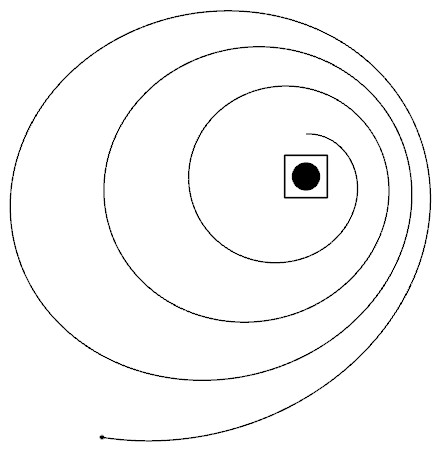
\includegraphics[width=0.95\textwidth]{pictures/sun_earth/euler_0_02.jpg}
        \caption{Expliziter Euler-Integrator}
      \end{subfigure}
      \begin{subfigure}[b]{0.49\textwidth}
        \center
        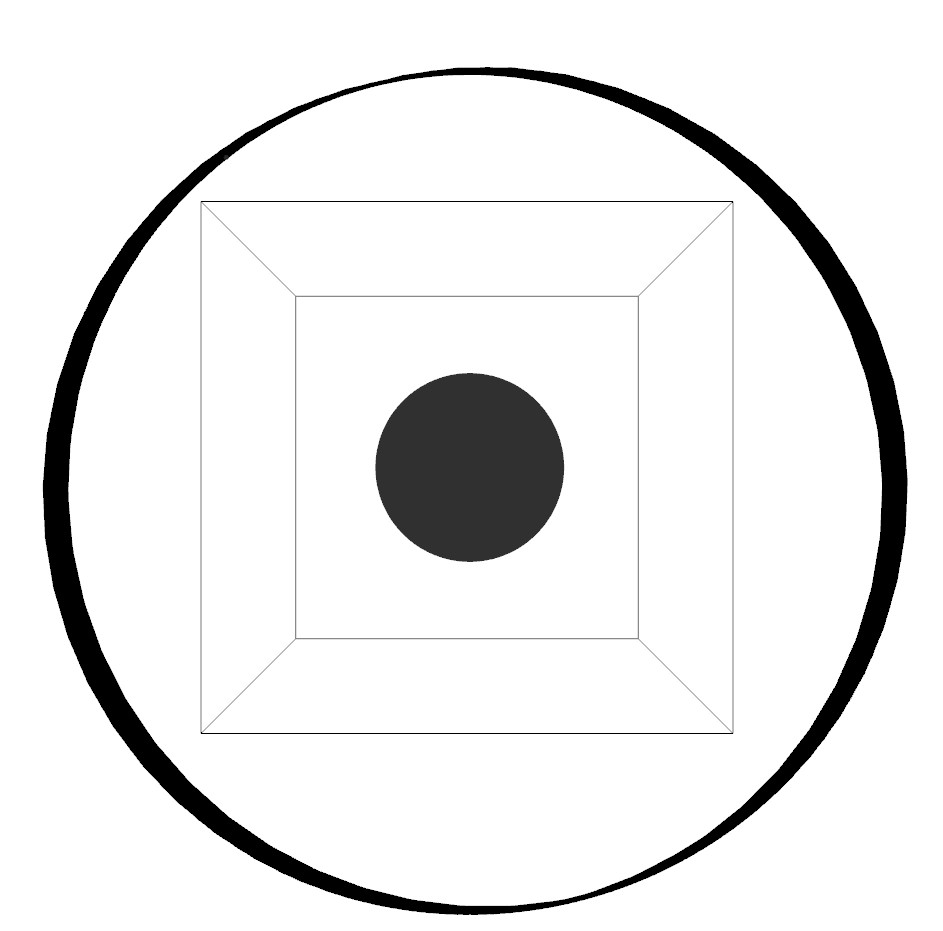
\includegraphics[width=0.95\textwidth]{pictures/sun_earth/seuler_0_02.jpg}
        \caption{Symplektischer Euler-Integrator}
      \end{subfigure}

      \begin{subfigure}[b]{0.49\textwidth}
        \center
        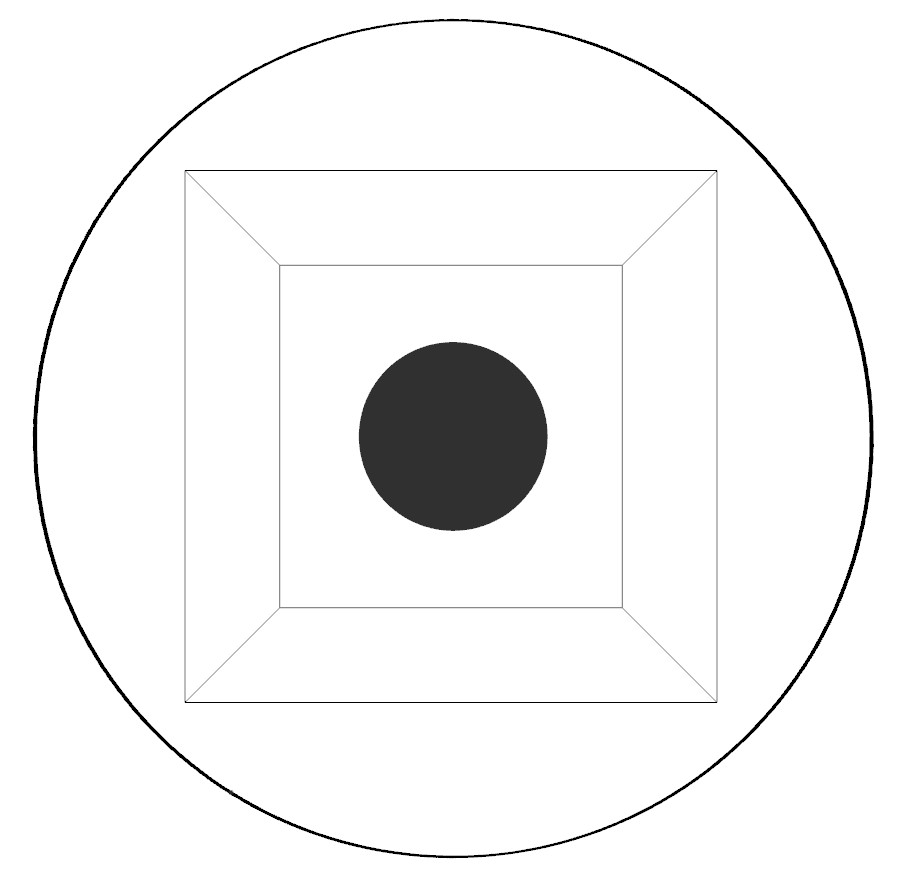
\includegraphics[width=0.95\textwidth]{pictures/sun_earth/leapfrog_0_02.jpg}
        \caption{Leapfrog-Integrator}
      \end{subfigure}
      \begin{subfigure}[b]{0.49\textwidth}
        \center
        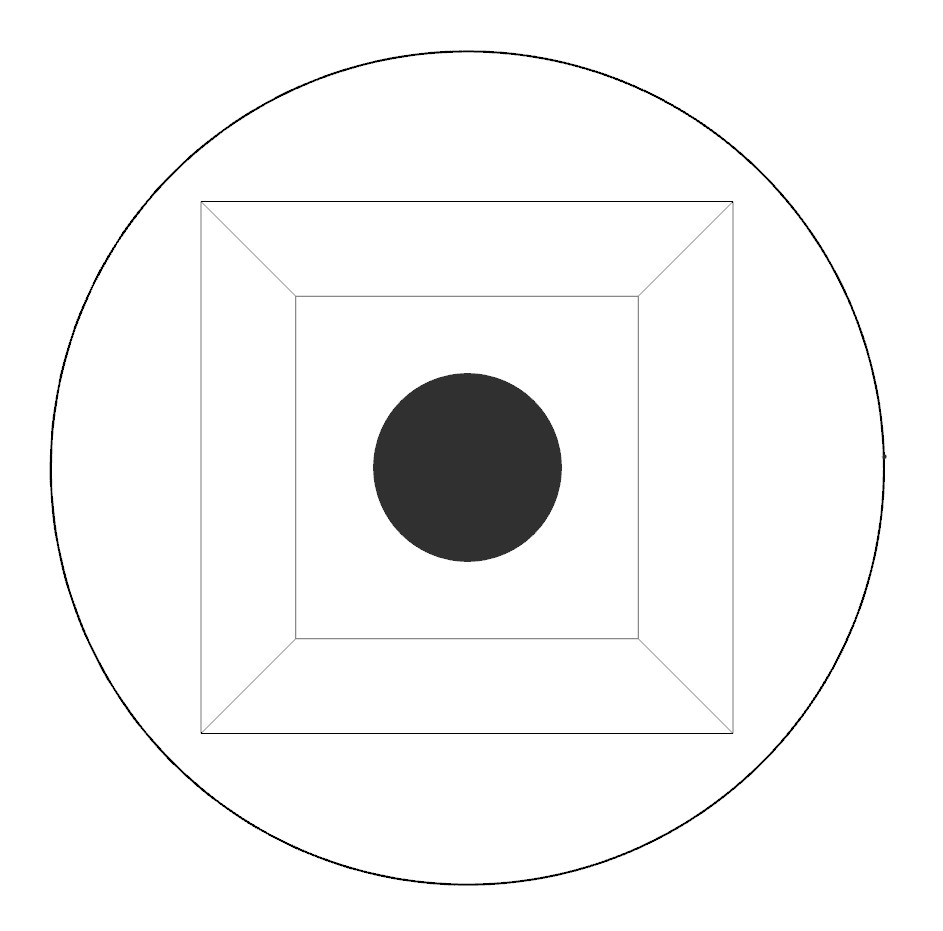
\includegraphics[width=0.95\textwidth]{pictures/sun_earth/rk4_0_02.jpg}
        \caption{RK4-Integrator}
      \end{subfigure}
      \caption{Die Abbildung zeigt den Verlauf der Bahnkurve der Erde in einem vereinfachten Sonne-Erde-System für verschiedene Integratoren mit einem Zeitschritt von $\Delta t = 0.020\,\m{a}$.}
      \label{fig:sun_earth2}
    \end{figure}

    \begin{figure}[p]
      \center
      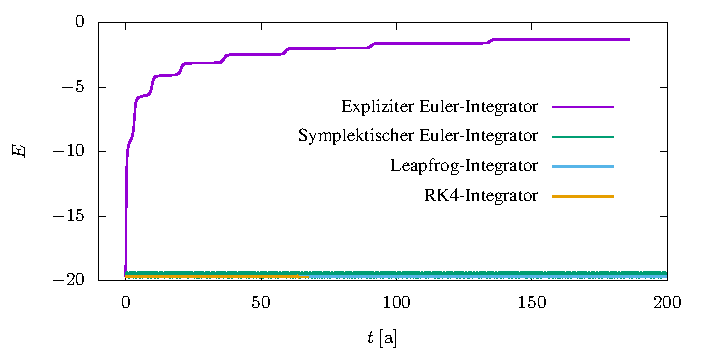
\includegraphics[width=0.95\textwidth]{plots/sun_earth_2_plot.pdf}
      \caption{Das Diagramm zeigt die Entwicklung der Gesamtenergie $E$ im Verlauf der Simulations-Zeit $t$ für verschiedene Integratoren mit einem festen Zeitschritt $\Delta t = 0.020$.}
      \label{fig:e2}
    \end{figure}

    \begin{figure}[h]
      \center
      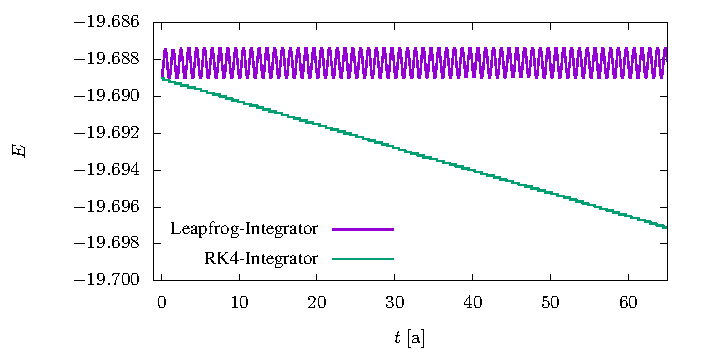
\includegraphics[width=0.95\textwidth]{plots/sun_earth_2_zoom_plot.pdf}
      \caption{Das Diagramm zeigt die Entwicklung der Gesamtenergie $E$ im Verlauf der Simulations-Zeit $t$ für verschiedene Integratoren mit einem festen Zeitschritt $\Delta t = 0.020$ und stellt zudem eine Vergrößerung des Diagrammes \ref{fig:e2} dar.}
      \label{fig:e2-zoom}
    \end{figure}

    In der grafischen Ausgabe sind die Unterschiede für einen kleineren Zeitschritt von $\Delta t = 0.02\,\m{a}$ zwischen Leapfrog- und dem RK4-Integrator nicht sichtbar.
    Beide erscheinen als perfekte Kreise und bestätigen die theoretischen Erwartungen.
    Allerdings sind in der Abbildung \ref{fig:e2-zoom}, die einen vergrößerten Bereich des Diagramms \ref{fig:e2} darstellt, durchaus geringe Unterschiede in beiden Verfahren erkennbar.
    Es wird deutlich, dass auch das Leapfrog-Verfahren Energieschwankungen aufweist, im Mittel dennoch die Energie erhält.
    Aufgrund der höheren Konvergenzordnung im Vergleich zum symplektischen Euler-Verfahren sind diese Schwankungen mehr als das zwanzigfache geringer.
    Das RK4-Verfahren arbeitet zwar mit einer Genauigkeit vierter Ordnung, ist aber nicht Energie-erhaltend.
    Wie in Abbildung \ref{fig:e2-zoom} zu erkennen, nimmt die Gesamtenergie über mehrere Iterationsschritte langsam ab, was bei einem expliziten Runge-Kutte-Integrator gerader Konvergenzordnung zu erwarten ist.
    Es muss sich demnach um ein instabiles Verfahren handeln.

    Die gezeigten Effekte werden durch die Wahl eines gröberen Zeitschrittes noch verstärkt.
    Abbildung \ref{fig:sun-earth-5} zeigt dasselbe Szenario für einen Zeitschritt von $\Delta t = 0.050\,\m{a}$.
    Das explizite Euler-Verfahren divergiert bereits nach einem fehlerhaften Umlauf.
    Die Instabilität des RK4-Verfahrens ist nun auch in der grafischen Ausgabe zu beobachten.
    Die Gesamtenergie nimmt im Laufe der Zeit ab, bis die Erde einen Minimalabstand zur Sonne unterschreitet und im darauffolgenden Integrationsschritt durch die Nähe zum Gravitationszentrum extrem beschleunigt wird und das System verlässt.
    Im Diagramm \ref{fig:e5} wird dieses Verhalten annähernd durch eine numerische Polstelle bei $t=200\,\m{a}$ beschrieben.
    Die beiden symplektischen Verfahren erhalten auch noch bei groben Zeitschritten die Gesamtenergie.
    In der grafischen Ausgabe äußern sich periodische Schwankungen der Energie durch periodische Schwankungen des Bahnradius.
    Die höhere Genauigkeit des Leapfrog-Verfahrens führt erneut zu einer Verringerung der Schwankungen gegenüber dem symplektischen Euler-Verfahren.

    \begin{figure}[p]
      \begin{subfigure}[b]{0.49\textwidth}
        \center
        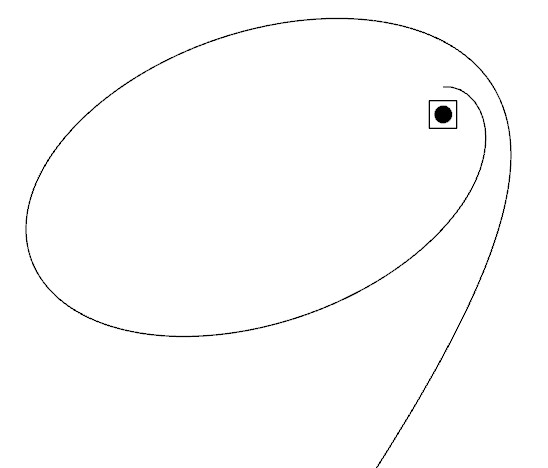
\includegraphics[width=0.95\textwidth]{pictures/sun_earth/euler_0_05.jpg}
        \caption{Expliziter Euler-Integrator}
      \end{subfigure}
      \begin{subfigure}[b]{0.49\textwidth}
        \center
        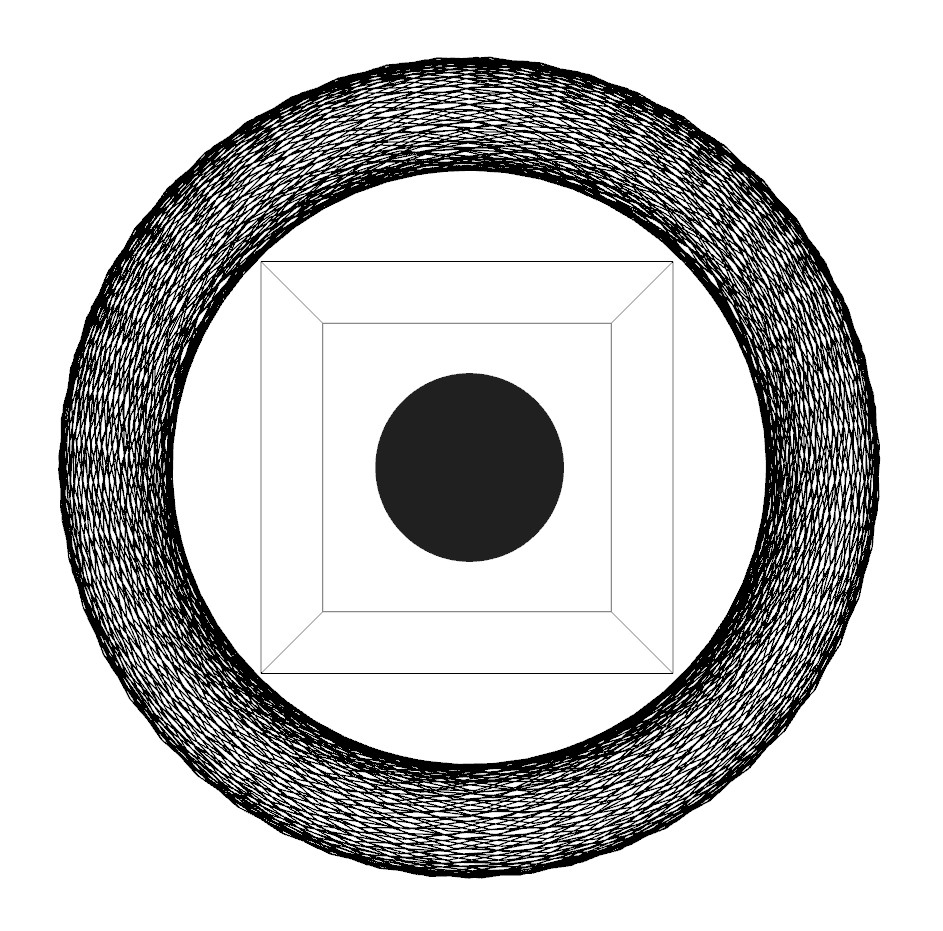
\includegraphics[width=0.95\textwidth]{pictures/sun_earth/seuler_0_05.jpg}
        \caption{Symplektischer Euler-Integrator}
      \end{subfigure}

      \begin{subfigure}[b]{0.49\textwidth}
        \center
        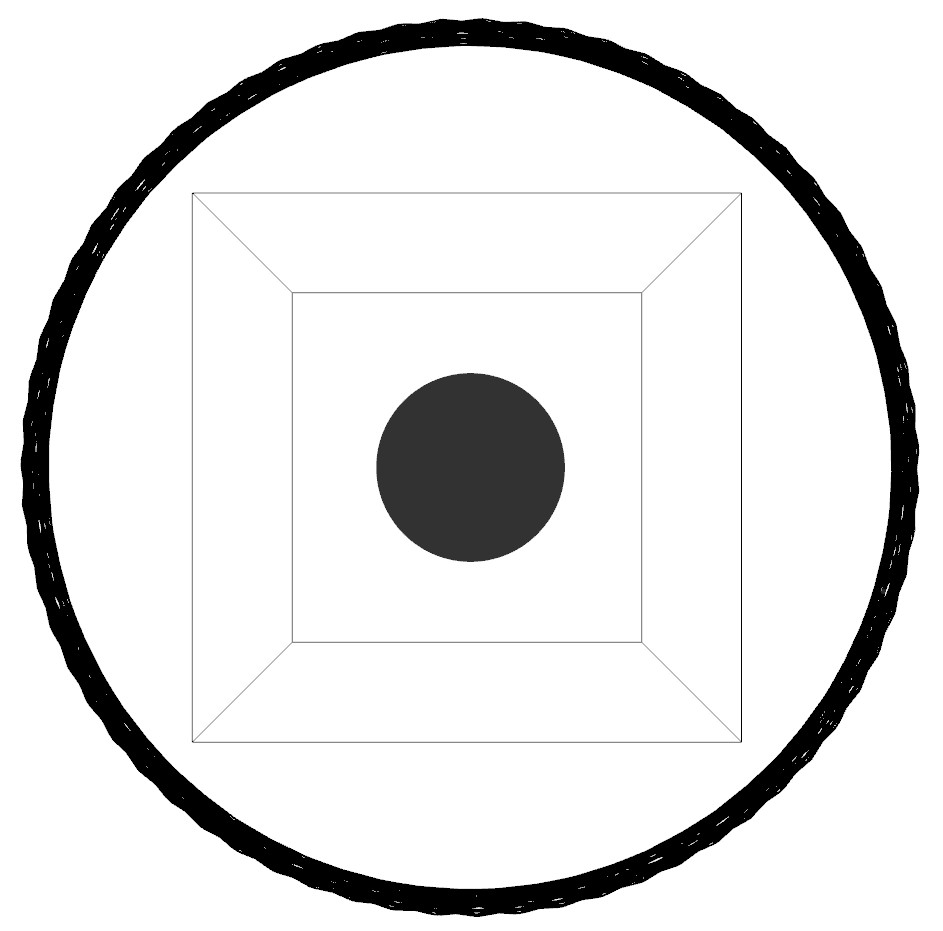
\includegraphics[width=0.95\textwidth]{pictures/sun_earth/leapfrog_0_05.jpg}
        \caption{Leapfrog-Integrator}
      \end{subfigure}
      \begin{subfigure}[b]{0.49\textwidth}
        \center
        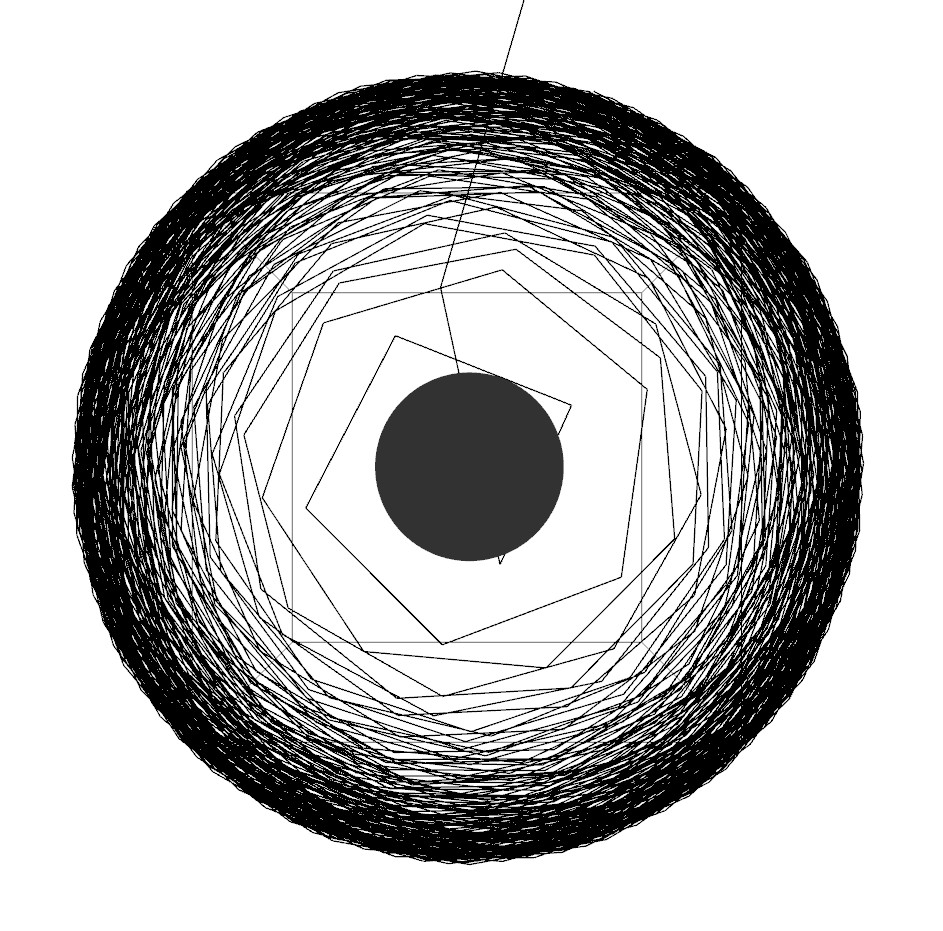
\includegraphics[width=0.95\textwidth]{pictures/sun_earth/rk4_0_05.jpg}
        \caption{RK4-Integrator}
      \end{subfigure}
      \caption{Die Abbildung zeigt den Verlauf der Bahnkurve der Erde in einem vereinfachten Sonne-Erde-System für verschiedene Integratoren mit einem Zeitschritt von $\Delta t = 0.050\,\m{a}$.}
      \label{fig:sun-earth-5}
    \end{figure}

    \begin{figure}[p]
      \center
      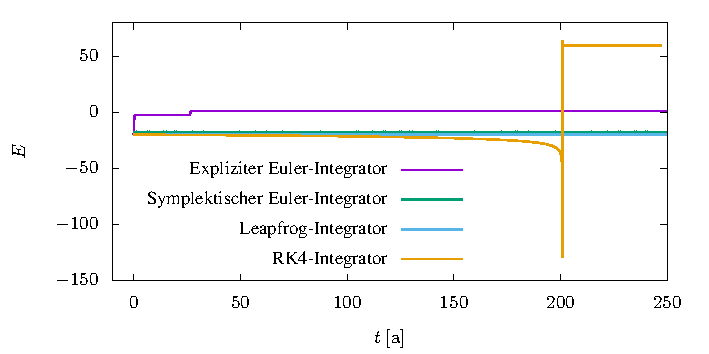
\includegraphics[width=0.95\textwidth]{plots/sun_earth_5_plot.pdf}
      \caption{Das Diagramm zeigt die Entwicklung der Gesamtenergie $E$ im Verlauf der Simulations-Zeit $t$ für verschiedene Integratoren mit einem festen Zeitschritt $\Delta t = 0.050$.}
      \label{fig:e5}
    \end{figure}

  % subsection stabilitätsanalyse (end)

  \subsection{Zweikörperproblem} % (fold)
  \label{sub:zweikörperproblem}

    Um die korrekte Funktionsweise der Integratoren zu überprüfen, haben wir, wie bereits in Abschnitt \ref{sub:das_zweikoerperproblem} erwähnt, analytisch lösbare Probleme simuliert.
    Vor allem das Zweikörperproblem stellt mit seiner Vielfalt an unterschiedlichen Lösungen eine ideale Testmöglichkeit dar.

    Die Lösungen des Zweikörperproblems teilen sich in gebundene und ungebundene Bewegungen ein.
    Abbildung \ref{fig:zkp-gebunden} zeigt diverse Beispiele dieser Bewegungen anhand eines Kreises, zweier sich nicht schneidender und zweier sich schneidender Ellipsen.
    Für das Szenario der konzentrischen Kreise in Abbildung \ref{subfig:konz-kreis} haben wir die Anfangswerte der beiden Massen so gesetzt, dass die Radialkräfte betragsmäßig gleich der Gravitationskraft zwischen beiden Punktmassen war.
    Den Schwerpunkt legten wir in den Koordinatenursprung.
    Für die beiden anderen Beispiele wählten kleinere Anfangsgeschwindigkeiten.
    \[
      m_1r_1 + m_2r_2 = 0
      \separate
      \frac{m_1\norm{v_1}^2}{\norm{r_1}} = \frac{\gamma m_1m_2}{\norm{r_1-r_2}^2} = \frac{m_2\norm{v_2}^2}{\norm{r_2}}
    \]
    \[
      \dotp{r_1}{v_1} = \dotp{r_2}{v_2} = 0
      \separate
      m_1v_1 + m_2v_2 = 0
    \]

    Die simulierten Partikelbahnen entsprechen somit den analytischen Lösungen und theoretischen Vorbetrachtungen.
    Dies spricht für die Genauigkeit der Integration.

    \begin{figure}
      \center
      \begin{subfigure}[b]{0.49\textwidth}
        \center
        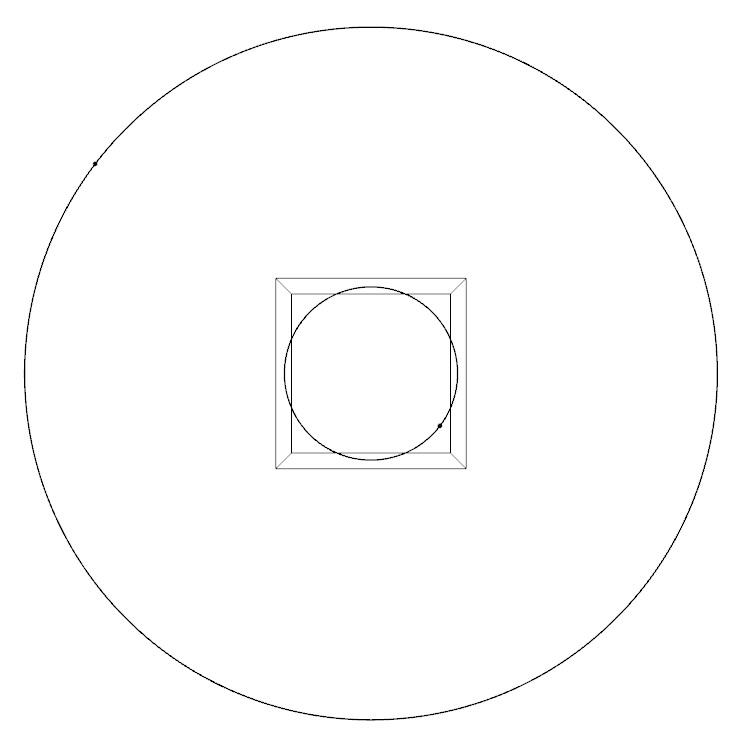
\includegraphics[width=0.95\textwidth]{pictures/two_body/circle.jpg}
        \caption{konzentrische Kreise}
        \label{subfig:konz-kreis}
      \end{subfigure}
      \begin{subfigure}[b]{0.49\textwidth}
        \center
        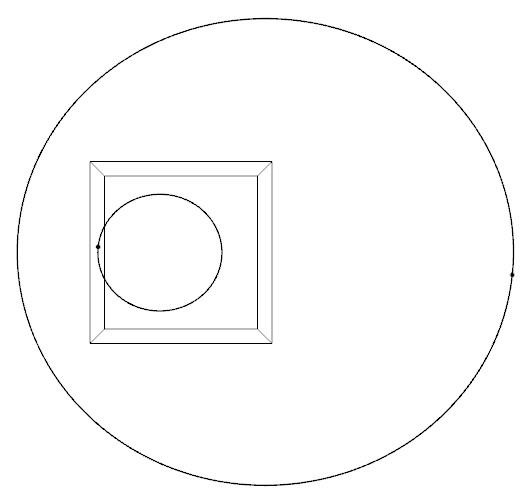
\includegraphics[width=0.95\textwidth]{pictures/two_body/ellipse_no-intersect.jpg}
        \caption{nicht-schneidende Ellipsen}
      \end{subfigure}

      \begin{subfigure}[b]{\textwidth}
        \center
        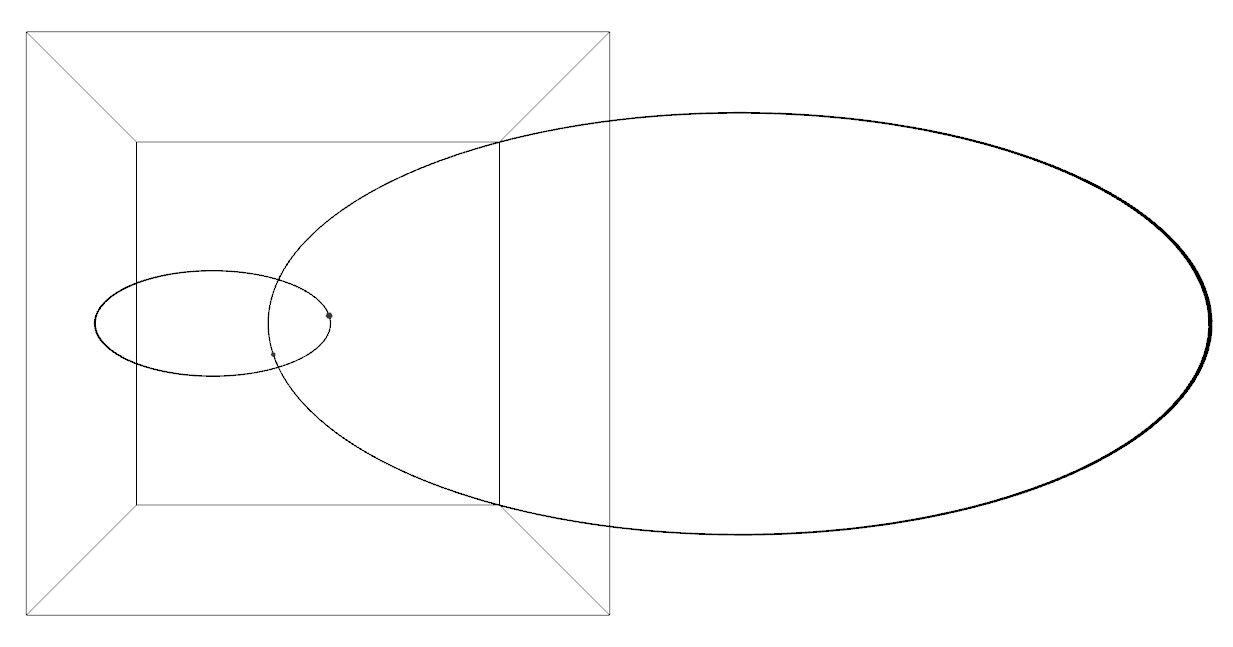
\includegraphics[width=0.95\textwidth]{pictures/two_body/ellipse_intersect.jpg}
        \caption{schneidende Ellipsen}
      \end{subfigure}
      \caption{Die Abbildung zeigt Beispiele für gebundene Bahnkurven des Zweikörperproblems. Die Bahnen wurden mithilfe des adaptiven Leapfrog-Integrators simuliert.}
      \label{fig:zkp-gebunden}
    \end{figure}

    In Abbildung \ref{fig:zkp-zykloide} zeigen wir zudem ein Beispiel, in welchem das Inertialsystem nicht dem Schwerpunktsystem gleicht, sondern eine konstante Relativgeschwindigkeit zu diesem aufweist.
    Wie zu erwarten, sind sogenannte Taumelbewegungen oder auch Zykloiden zu beobachten.

    \begin{figure}[h]
      \center
      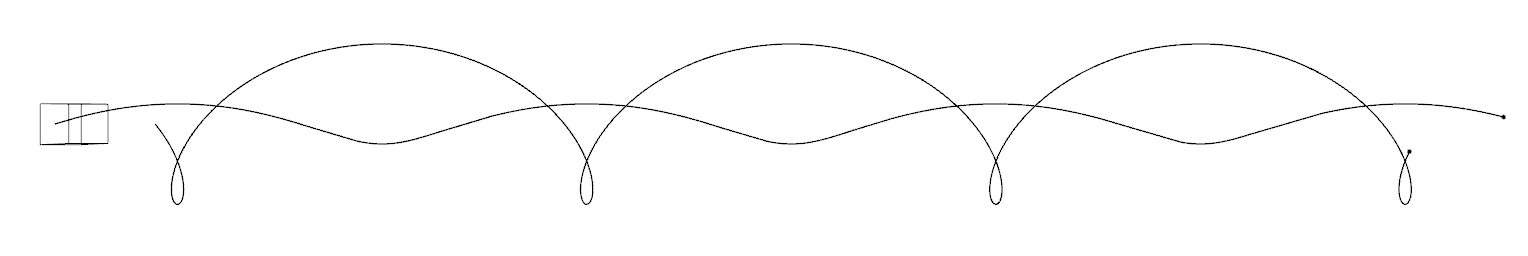
\includegraphics[width=0.95\textwidth]{pictures/two_body/cycloid.jpg}
      \caption{Die Abbildung zeigt ein Beispiel für eine gebundene Bahnkurven des Zweikörperproblems aus Sicht eines nicht im Schwerpunkt verankerten Inertialsystems. Es bilden sich typische Zykloide. Die Bahnen wurden mithilfe des adaptiven Leapfrog-Integrators simuliert.}
      \label{fig:zkp-zykloide}
    \end{figure}

    Die unbeschränkten Lösungen des Zweikörperproblems sind in den Beispielen in Abbildung \ref{fig:zkp-ungebunden} zu sehen.
    Man unterscheidet diese nach ihrer Exzentrizität $\varepsilon$.
    Für $\varepsilon = 1$ ergibt sich der Spezialfall einer Parabel, der erreicht werden kann, indem man die Anfangswerte der Punktmassen anpasst, sodass für die Gesamtenergie $E=0$ gilt.
    Für positive Energien ergeben sich Hyperbel-Bahnen, die sich im Unendlichen einer Gerade annähern.
    Alle genannten Eigenschaften konnten in unserer Simulation nicht nur qualitativ, sondern auch quantitativ bestätigt werden.

    \begin{figure}[h]
      \center
      \begin{subfigure}[b]{0.49\textwidth}
        \center
        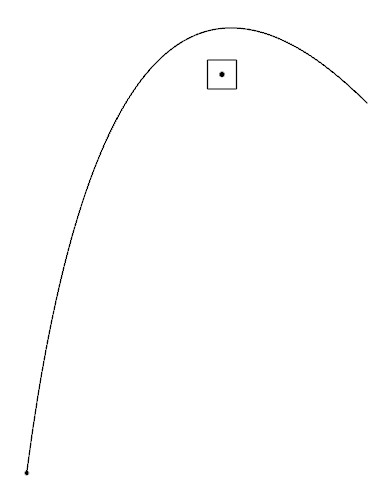
\includegraphics[width=0.95\textwidth]{pictures/two_body/parabel.jpg}
        \caption{Parabel ($\varepsilon=1$)}
      \end{subfigure}
      \begin{subfigure}[b]{0.49\textwidth}
        \center
        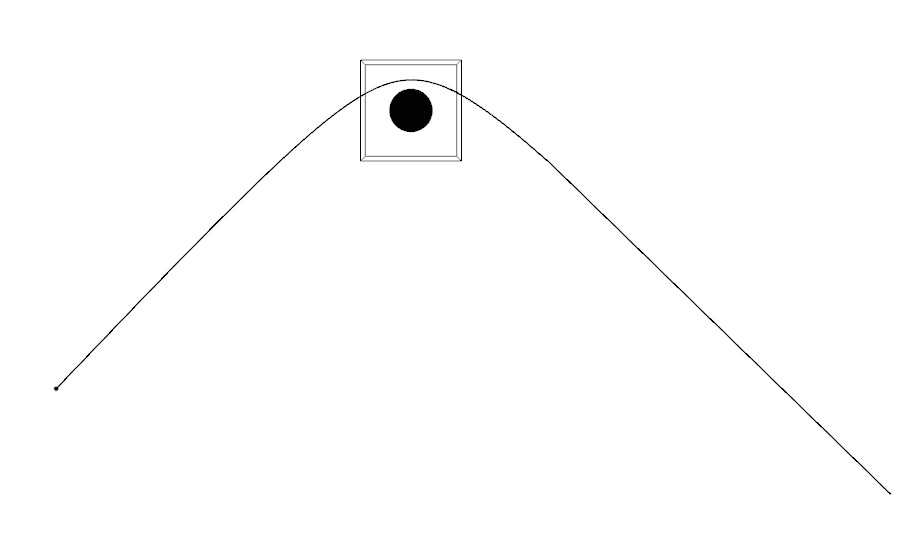
\includegraphics[height=0.95\textwidth,angle=90]{pictures/two_body/hyperbol.jpg}
        \caption{Hyperbel ($\varepsilon >1$)}
      \end{subfigure}
      \caption{Die Abbildung zeigt Beispiele für nicht-gebundene Bahnkurven des Zweikörperproblems. Die Bahnen wurden mithilfe des adaptiven Leapfrog-Integrators simuliert.}
      \label{fig:zkp-ungebunden}
    \end{figure}

  % subsection zweikörperproblem (end)

  \subsection{Dreikörperproblem} % (fold)
  \label{sub:dreikörperproblem}

    Für das Dreikörperproblem gibt eine Vielzahl analytischer Lösungen für Spezialfälle.
    Wir wählten eine simplen Fall, bei dem die drei Punktmassen drei identische Kreisbahnen verfolgten.
    Dafür setzten wir die Anfangswerte der Massen, sodass der Betrag der Radialkraft jeder einzelnen Masse dem Betrag der Summe der Gravitationskräfte der übrigen Massen entsprach.
    Zudem positionierten wir die Punktmassen auf einem gleichseitigen Dreieck.

    In Abbildung \ref{fig:dkp} ist diese Anordnung und ihr zeitlicher Verlauf simuliert worden.
    Nach circa zweieinhalb Umdrehungen innerhalb von $7.5\,\m{a}$, die der geschlossenen Lösung entsprachen, begannen merkbare numerische Rundungsfehler zu erscheinen, wie sie bei $t=9.1\,\m{a}$ zu sehen sind.
    Diese verstärkten sich im folgenden Verlauf und führten zu immer größeren Asymmetrien.
    Nach fortgeschrittener Zeit erschien die Bewegung chaotisch.
    Wir schließen daraus, dass es sich bei dem berechneten Spezialfall nur um ein instabiles Gleichgewicht handeln kann.
    Kleinste Fehler, hier erzeugt durch Gleitkommaarithmetik, gleichen sich demnach nicht aus und divergieren.

    \begin{figure}[h]
      \center
      \begin{subfigure}[b]{0.49\textwidth}
        \center
        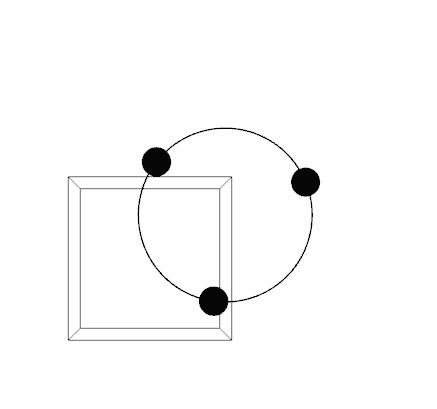
\includegraphics[width=0.95\textwidth]{pictures/three_body/triangle_1.jpg}
        \caption{$t=3.3\,\m{a}$}
      \end{subfigure}
      \begin{subfigure}[b]{0.49\textwidth}
        \center
        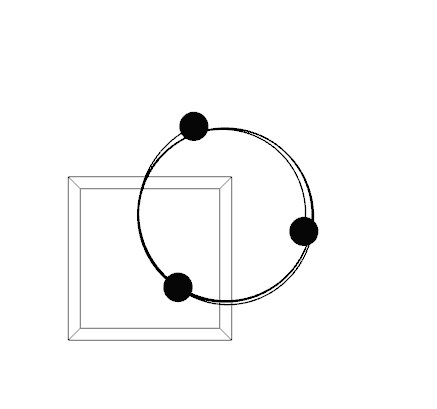
\includegraphics[width=0.95\textwidth]{pictures/three_body/triangle_2.jpg}
        \caption{$t=9.1\,\m{a}$}
      \end{subfigure}

      \begin{subfigure}[b]{0.49\textwidth}
        \center
        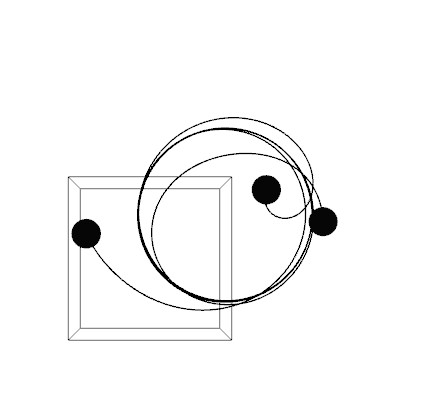
\includegraphics[width=0.95\textwidth]{pictures/three_body/triangle_3.jpg}
        \caption{$t=10.9\,\m{a}$}
      \end{subfigure}
      \begin{subfigure}[b]{0.49\textwidth}
        \center
        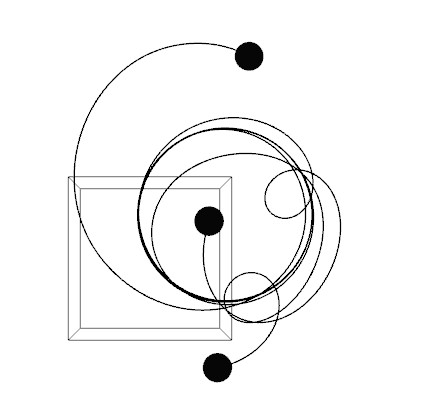
\includegraphics[width=0.95\textwidth]{pictures/three_body/triangle_4.jpg}
        \caption{$t=13.5\,\m{a}$}
      \end{subfigure}

      \begin{subfigure}[b]{0.49\textwidth}
        \center
        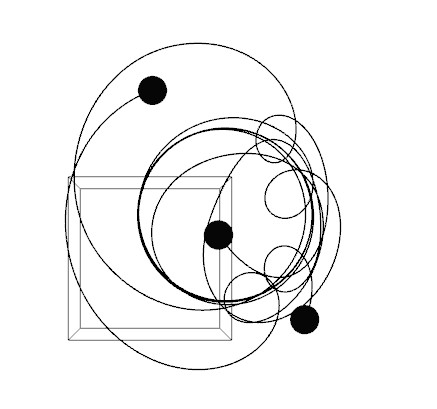
\includegraphics[width=0.95\textwidth]{pictures/three_body/triangle_5.jpg}
        \caption{$t=16.8\,\m{a}$}
      \end{subfigure}
      \begin{subfigure}[b]{0.49\textwidth}
        \center
        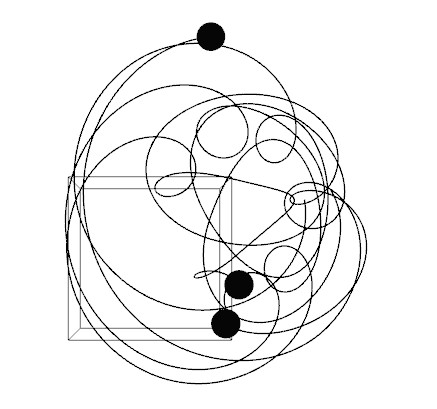
\includegraphics[width=0.95\textwidth]{pictures/three_body/triangle_6.jpg}
        \caption{$t=23.0\,\m{a}$}
      \end{subfigure}
      \caption{Die Abbildung zeigt den numerischen Verlauf der Bahnen eines Spezialfalls des Dreikörperproblems, dessen analytische Lösung drei identische Kreisbahnen wie im ersten Bild beschreibt. Die numerischen Fehler verstärken sich im Laufe der Zeit und führen somit zu chaotischen Bahnen. Es wurde das Leapfrog-Verfahren mit einem festen Zeitschritt von $\Delta t = 5\cdot 10^{-4}\,\m{a}$ verwendet.}
      \label{fig:dkp}
    \end{figure}

  % subsection dreikörperproblem (end)

  \subsection{Laufzeitanalyse} % (fold)
  \label{sub:laufzeitanalyse}

    Obwohl es beim Implementieren der Integratoren hauptsächlich um deren Stabilität und Genauigkeit ging, ist es für das spätere adaptive Zeitschrittverfahren relevant eine Performance-Analyse durchzuführen.
    Hierfür verwendeten wir für alle verfügbaren Integratoren ein System, bestehend aus $2000$ Punktmassen mit einer Zentralmasse.
    Die Berechnungsschritte pro Sekunde wurden vom Computer gemessen und ausgegen.
    Sie sind in Tabelle \ref{tab:fps} gegeben.

    \begin{table}[h]
      \caption{Die Tabelle zeigt die Iterationsschritte pro Sekunde (FPS) eines jeden Integrators, gemessen auf dem gleichen Computersystem, um diese miteinander zu vergleichen. Die Szene wurde durch $2000$ Punktmassen mit einer Zentralmasse beschrieben.}
      \label{tab:fps}
      \center
      \begin{tabular}{lcccc}
        \hline
        \hline
        Integrator & expliziter Euler & symplektischer Euler & Leapfrog & RK4 \\
        \hline
        FPS & $41$ & $41$ & $27$ & $17$ \\
        \hline
        \hline
      \end{tabular}
    \end{table}

    Wie zu erwarten, liefern die beiden Euler-Verfahren aufgrund ihrer ähnlichen und simplen Struktur, die maximale Performance unter den gemessenen Verfahren.
    Der Leapfrog-Integrator ist aufgrund seiner höheren Konvergenzordnung, welche einen komplizierteren Algorithmus zur Folge hat, langsamer.
    Analoges gilt für das RK4-Verfahren, welches algorithmisch gesehen das Aufwendigste der vewendeten Verfahren darstellt.

    Allerdings ist die Performance der Integratoren nicht ausschlaggebend, sobald sie zusammen mit einem adaptiven Zeitschrittverfahren verwendet werden.
    Es stellte sich heraus, dass für eine adaptive Wahl des Zeitschrittes ein Optimum aus Performance und Genauigkeit entscheidend war.
    So erschien das RK4-Verfahren trotz seines hohen Rechenaufwands dem expliziten Euler-Integrator weit überlegen, da die Schrittweitensteuerung wesentlich größere Zeitschritte verwendete.
    Die Zeit innerhalb der Simulation konnte somit schneller durchlaufen werden.

  % subsection laufzeitanalyse (end)

  \subsection{Simulation des Sonnensystems} % (fold)
  \label{sub:simulation_des_sonnensystems}

    Die absolute Kultaufgabe und Must-Have einer $n$-Körper-Simulation ist die Simulation des eigenen Sonnensystems.
    Deswegen widmeten auch wir uns dieser Aufgabe.
    Wir haben uns bewusst dazu entschieden, Pluto in die Planetensimulation mit einzubeziehen, da wir seine Ausgrenzung nicht unterstützen.
    Es sollte nicht immer auf die Größe ankommen.
    Für die Anfangswerte der Sonne und aller Planeten verwendeten wir bekannte Ephemeriden, siehe \ref{sec:ephemeriden_des_sonnensystem}.
    Ein beispielhafte grafische Ausgabe ist in Abbildung \ref{fig:solarsystem} gezeigt.
    Die Betrachtung dieser weckt heimatliche Gefühle.

    Um die Genauigkeit der Simulation anhand des Sonnensystems zu überprüfen, bestimmten wir die Mittelwerte diverser Kenngrößen aller Planeten im Sonnensystem.
    In Tabelle \ref{tab:solarsystem} sind diese Werte zusammen mit ihren bekannten Literaturwerten dargestellt.
    Der Vergleich mit den bekannten Literatur zeigt eine bemerkenswerte Übereinstimmung aller Werte.

    \begin{figure}[h]
      \center
      \begin{subfigure}[b]{0.49\textwidth}
        \center
        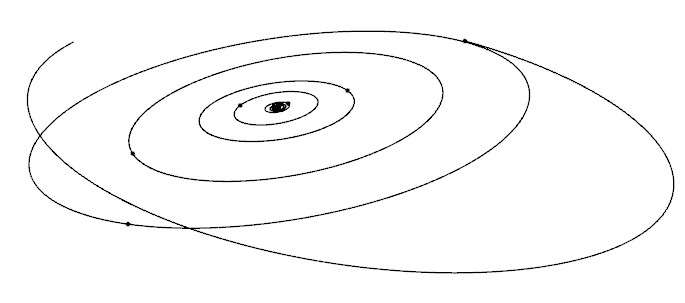
\includegraphics[width=0.95\textwidth]{pictures/solar_system/total.jpg}
        \caption{gesamtes Sonnensystem}
      \end{subfigure}
      \begin{subfigure}[b]{0.49\textwidth}
        \center
        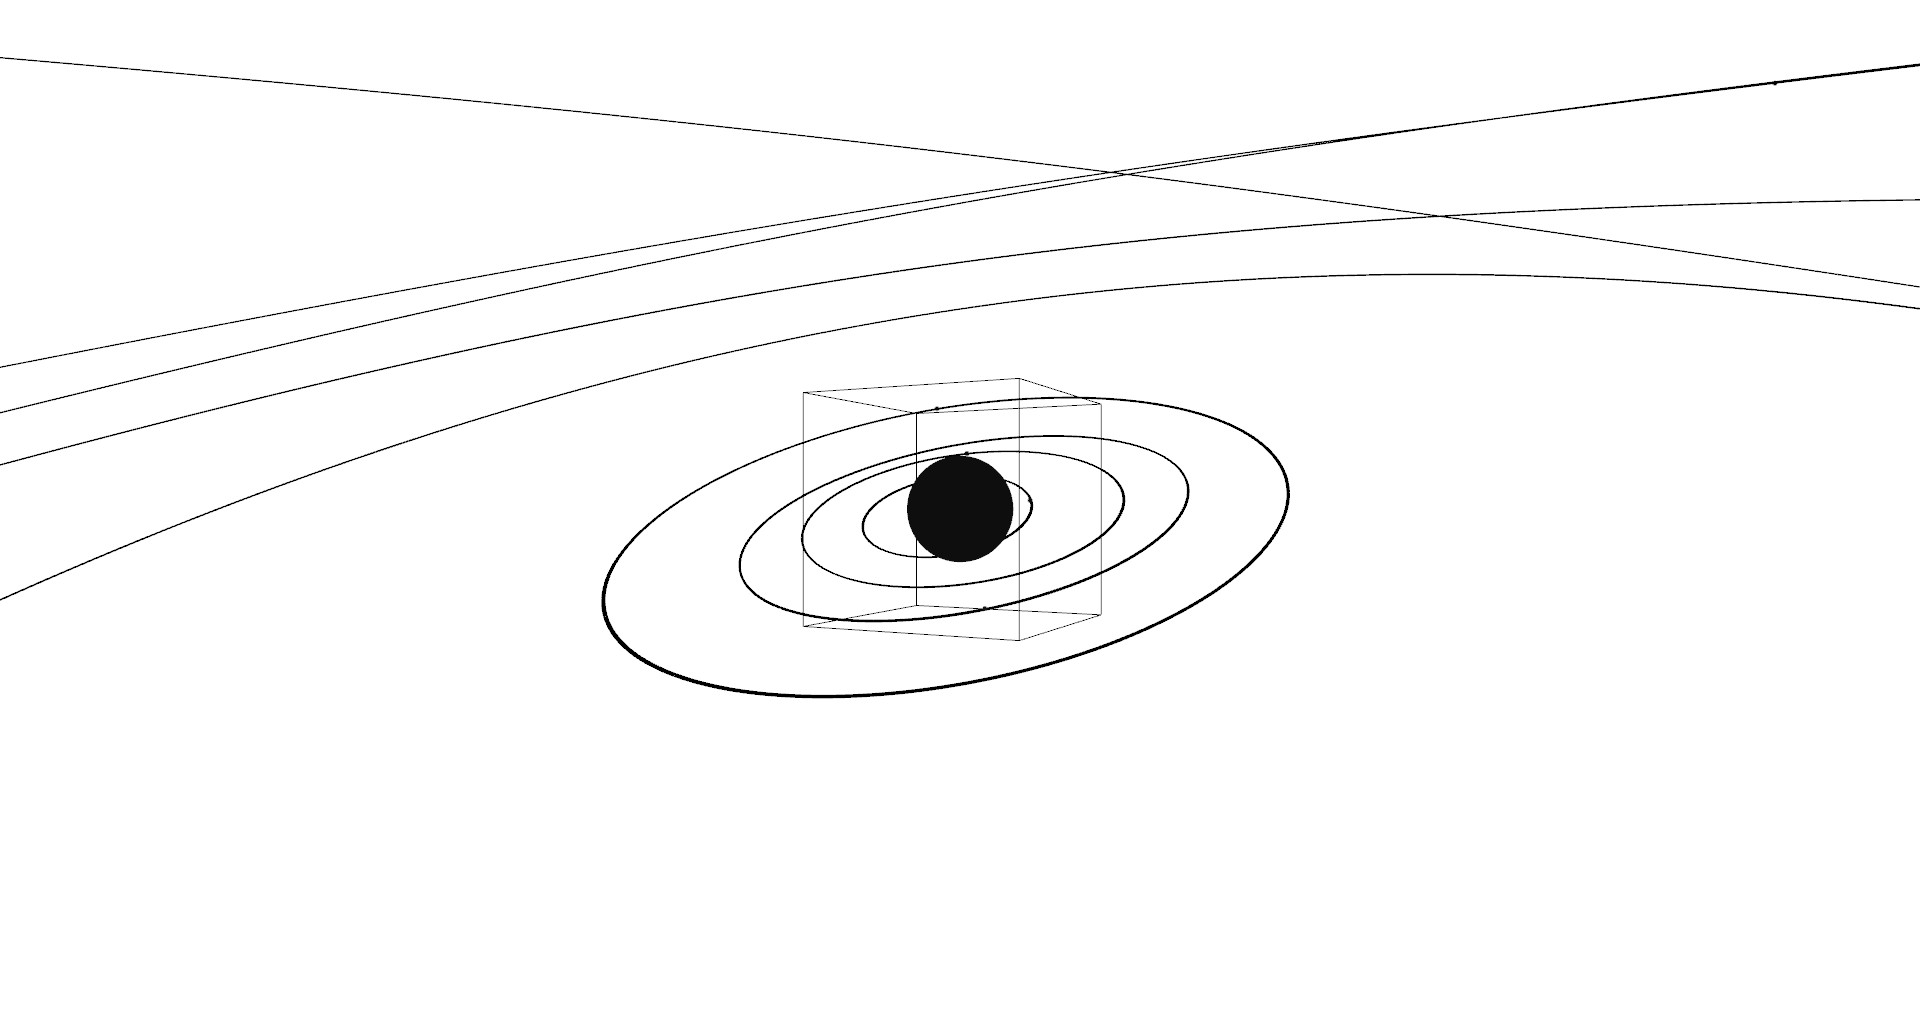
\includegraphics[width=0.95\textwidth]{pictures/solar_system/zoom.jpg}
        \caption{innere Planetenbahnen}
      \end{subfigure}
      \caption{Die Abbildung zeigt eine Simulation des Sonnensystems basierend auf Ephemeriden. Die Berechnung erfolgten unter Verwendung des adaptiven Leapfrog-Verfahrens.}
      \label{fig:solarsystem}
    \end{figure}

    \urldef{\solarsystemdata}\url{https://de.wikipedia.org/wiki/Liste_der_Planeten_des_Sonnensystems}
    \urldef{\plutodata}\url{https://en.wikipedia.org/wiki/Pluto}
    \begin{table}[h]
      \center
      \caption{Die Tabelle zeigt simulierte und tabellarische Kennwerte der Planeten unseres Sonnensystems. Dabei bezeichnet $T$ die Umlaufzeit, $a$ die große Halbachse und $\varepsilon$ die Exzentrizität. Zugehörige Tabellenwerte sind durch den Index $\m{Tab}$ gekennzeichnet. \\ Quelle: \\ \solarsystemdata \\ \plutodata}
      \label{tab:solarsystem}
      \renewcommand{\arraystretch}{1.5}
      \begin{tabular}{l|rr|rr|rr}
        \hline
        Planeten & $T \ [\m{a}]$ & $T_\m{Tab}\ [\m{a}]$ & $a \ [\m{AE}]$ & $a_\m{Tab} \ [\m{AE}]$ & $\varepsilon$ & $\varepsilon_\m{Tab}$ \\
        \hline
        \hline
        Merkur & $0.241$ & $0.2410$ & $0.387$ & $0.387$ & $0.201$ & $0.206$ \\
        Venus & $0.616$ & $0.6156$ & $0.723$ & $0.723$ & $0.00639$ & $0.00677$ \\
        Erde & $1.001$ & $1.000$ & $0.999$ & $1.00$ & $0.0161$ & $0.0167$ \\
        Mars & $1.880$ & $1.882$ & $1.52$ & $1.52$ & $0.0939$ & $0.0934$ \\
        Jupiter & $11.85$ & $11.86$ & $5.20$ & $5.20$ & $0.0495$ & $0.0484$ \\
        Saturn & $29.40$ & $29.46$ & $9.56$ & $9.54$ & $0.0554$ & $0.0542$ \\
        Uranus & $84.07$ & $84.01$ & $19.2$ & $19.19$ & $0.0464$ & $0.0472$ \\
        Neptun & $164.9$ & $164.8$ & $30.1$ & $30.06$ & $0.00878$ & $0.00859$ \\
        Pluto & $247.9$ & $247.9$ & $39.6$ & $39.48$ & $0.250$ & $0.249$ \\
        \hline
        \hline
      \end{tabular}
    \end{table}

  % subsection simulation_des_sonnensystems (end)

  \subsection{Wahl des Zeitschrittes} % (fold)
  \label{sub:wahl_des_zeitschrittes}

    Komplizierte $n$-Körper-Probleme sind nicht nur aufwendig zu simulieren, sondern erfordern auch einen gut-gewählten Zeitschritt.
    Einen Zeitschritt im Vorfeld zu bestimmen, ist eine nicht-triviale Aufgabe und oft nicht praxistaugliches Verfahren.
    Das Setzen eines konstanten Zeitschrittes führt zudem notwendigerweise zu der Wahl einer sehr kleinen Schrittweite.
    Der Rechenaufwand und die damit benötigte Simulationszeit steigt damit erheblich, ohne sicher zu stellen, dass die Simulation in allen Schritten korrekt verläuft.
    Wie in Abschnitt \ref{sub:adaptiver_zeitschritt} beschrieben, konnten wir zeigen, dass die Wahl eines adaptiven Zeitschrittes überlegen zu den vorher genannten Methoden ist.
    Abbildung \ref{fig:20-koerper} stellt ein System von zwanzig Massen mit einem schweren Zentralkörper dar.
    Ein solches System benötigt je nach Anordnung und Zeitpunkt unterschiedliche Zeitschritte, da ansonsten die Bahnen der Planeten stark verfälscht werden, wie es in Abbildung \ref{subfig:20-koerper-konst} gezeigt ist.
    Der Zeitschritt war für einige der inneren Punktmassen zu grob gewählt und führte der Charakteristik des RK4-Verfahrens folgend zu Implosionen der Bahnen.
    Äußere Planeten zeigten jedoch keine sichtbaren Fehler und hätten mit einer noch größeren Schrittweite berechnet werden können.
    Durch Verwendung eines adaptiven Verfahrens konnten wir dergleichen verhindern.
    Abbildung zeigt \ref{subfig:20-koerper-adap} zeigt das gleiche System mit stabilen Bahnverläufen.
    Die gewählten Zeitschritte des Algorithmus lagen in dem Bereich $[0.0005\,\m{a},0.08\,\m{a}]$.
    Interessant ist dabei, dass der zuvor gewählte Zeitschritt innerhalb des gegebenen Intervalls liegt und nicht zu grob gewählt scheint.
    Dennoch scheinen kritische Zeitpunkte zu existieren, an denen die Wahl einer kleineren Schrittweite unerlässlich ist.
    Die Wahl einer Computer-gestützten Schrittweite sollte aus diesen Gründen der Wahl einer konstanten Schrittweise immer bevorzugt werden.

    \begin{figure}[h]
      \begin{subfigure}[b]{0.49\textwidth}
        \center
        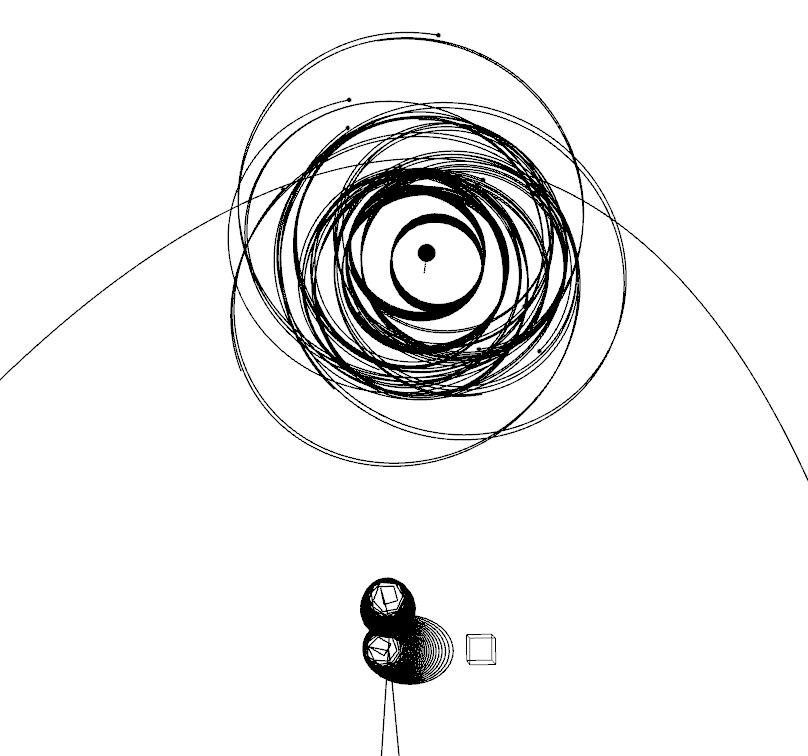
\includegraphics[width=0.95\textwidth]{pictures/adaptive/shit.jpg}
        \caption{konstanter Zeitschritt $\Delta t = 0.070\,\m{a}$}
        \label{subfig:20-koerper-konst}
      \end{subfigure}
      \begin{subfigure}[b]{0.49\textwidth}
        \center
        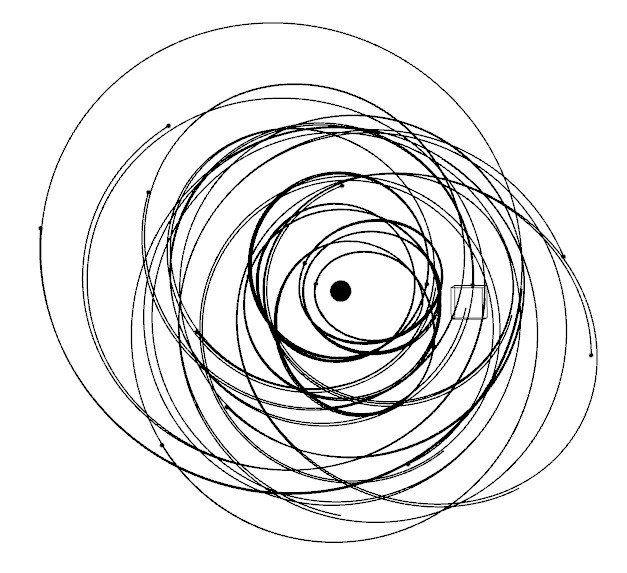
\includegraphics[width=0.95\textwidth]{pictures/adaptive/good.jpg}
        \caption{adaptiver Zeitschritt}
        \label{subfig:20-koerper-adap}
      \end{subfigure}
      \caption{Die Abbildung zeigt eine $n$-Körper-Simulation mit $n=20$ für unterschiedliche Zeitschrittverfahren und einem RK4-Integrator. Das adaptive Verfahren zeigt keine divergierenden Bahnen im Gegensatz zur konstanten Zeitschrittwahl.}
      \label{fig:20-koerper}
    \end{figure}

  % subsection wahl_des_zeitschrittes (end)

  % \subsection{Vergleich mit Mercury6} % (fold)
  % \label{sub:vergleich_mit_mercury6}

  %   \begin{itemize}
  %     \item wahl eines einfachen systems
  %     \item vergleich der halbachse der erde
  %   \end{itemize}

  % subsection vergleich_mit_mercury6 (end)

% section ergebnisse (end)